\newpage
\hypertarget{initialize tex}{}
\subsection{First steps}
\texHeader

In your Eclipse workspace, find and open \texttt{Dictionary/MOSL/\_imports.mconf} (Fig.~\ref{eclipse:standardImports}). You'll notice that it's already
accessing the \texttt{MocaTree} and some other built-in metamodels -- you're already able to start with both metamodels.

\vspace{0.5cm}

\begin{figure}[htbp]
\begin{center}
  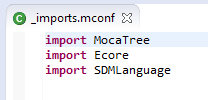
\includegraphics[width=0.4\textwidth]{eclipse_importsFile}
  \caption{\texttt{Dictionary}'s imports file}
  \label{eclipse:standardImports}
\end{center}
\end{figure}

\begin{enumerate}

\item[$\blacktriangleright$] Let's create the TGG we'll use to transform \texttt{MocaTree} to \texttt{Dictionary}. Right-click on \texttt{MyWorkingSet}, and
navigate to ``New/ TGG.''

\item[$\blacktriangleright$] Name the package \texttt{DictionaryCodeAdapter}, setting the source as \texttt{MocaTree} and target as \texttt{DictionaryLanguage}
(Fig.~\ref{eclipse:newTGGProject}).

\begin{figure}[htbp]
\begin{center}
  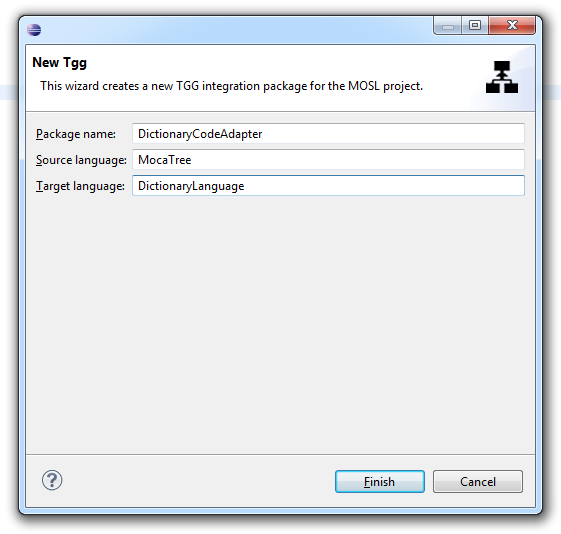
\includegraphics[width=0.9\textwidth]{eclipse_dictionaryCodeAdapterTGGProject}
  \caption{Settings for our TGG}
  \label{eclipse:newTGGProject}
\end{center}
\end{figure}

\item[$\blacktriangleright$] A \texttt{schema.sch} file should automatically open in the editor. As a first step, let's add a correspondence type
between \texttt{Folder} and \texttt{Library} as depicted in Fig~\ref{eclipse:firstSchema}.\footnote{For details on this correspondence metamodel and how to
create types, refer to Part IV, Section 3.} Don't forget that you can use eMoflon's auto-completion feature here!

\begin{figure}[htbp]
\begin{center}
  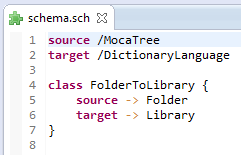
\includegraphics[width=0.5\textwidth]{eclipse_schemaStart}
  \caption{Our first correspondence type}
  \label{eclipse:firstSchema}
\end{center}
\end{figure}

\item[$\blacktriangleright$] Save and build your project. Confirm that the generated project has a solid black hexagon symbol overlaying the folder, indicating
\texttt{DictionaryCodeAdapter} is a TGG project, and not just a standard Ecore project (the default project type).

\end{enumerate}
